% Options for packages loaded elsewhere
\PassOptionsToPackage{unicode}{hyperref}
\PassOptionsToPackage{hyphens}{url}
%
\documentclass[
  a4paper,
  11pt,
  twocolumn]{article}
\usepackage{amsmath,amssymb}
\usepackage{iftex}
\ifPDFTeX
  \usepackage[T1]{fontenc}
  \usepackage[utf8]{inputenc}
  \usepackage{textcomp} % provide euro and other symbols
\else % if luatex or xetex
  \usepackage{unicode-math} % this also loads fontspec
  \defaultfontfeatures{Scale=MatchLowercase}
  \defaultfontfeatures[\rmfamily]{Ligatures=TeX,Scale=1}
\fi
\usepackage{lmodern}
\ifPDFTeX\else
  % xetex/luatex font selection
\fi
% Use upquote if available, for straight quotes in verbatim environments
\IfFileExists{upquote.sty}{\usepackage{upquote}}{}
\IfFileExists{microtype.sty}{% use microtype if available
  \usepackage[]{microtype}
  \UseMicrotypeSet[protrusion]{basicmath} % disable protrusion for tt fonts
}{}
\makeatletter
\@ifundefined{KOMAClassName}{% if non-KOMA class
  \IfFileExists{parskip.sty}{%
    \usepackage{parskip}
  }{% else
    \setlength{\parindent}{0pt}
    \setlength{\parskip}{6pt plus 2pt minus 1pt}}
}{% if KOMA class
  \KOMAoptions{parskip=half}}
\makeatother
\usepackage{xcolor}
\usepackage{color}
\usepackage{fancyvrb}
\newcommand{\VerbBar}{|}
\newcommand{\VERB}{\Verb[commandchars=\\\{\}]}
\DefineVerbatimEnvironment{Highlighting}{Verbatim}{commandchars=\\\{\}}
% Add ',fontsize=\small' for more characters per line
\usepackage{framed}
\definecolor{shadecolor}{RGB}{48,48,48}
\newenvironment{Shaded}{\begin{snugshade}}{\end{snugshade}}
\newcommand{\AlertTok}[1]{\textcolor[rgb]{1.00,0.81,0.69}{#1}}
\newcommand{\AnnotationTok}[1]{\textcolor[rgb]{0.50,0.62,0.50}{\textbf{#1}}}
\newcommand{\AttributeTok}[1]{\textcolor[rgb]{0.80,0.80,0.80}{#1}}
\newcommand{\BaseNTok}[1]{\textcolor[rgb]{0.86,0.64,0.64}{#1}}
\newcommand{\BuiltInTok}[1]{\textcolor[rgb]{0.80,0.80,0.80}{#1}}
\newcommand{\CharTok}[1]{\textcolor[rgb]{0.86,0.64,0.64}{#1}}
\newcommand{\CommentTok}[1]{\textcolor[rgb]{0.50,0.62,0.50}{#1}}
\newcommand{\CommentVarTok}[1]{\textcolor[rgb]{0.50,0.62,0.50}{\textbf{#1}}}
\newcommand{\ConstantTok}[1]{\textcolor[rgb]{0.86,0.64,0.64}{\textbf{#1}}}
\newcommand{\ControlFlowTok}[1]{\textcolor[rgb]{0.94,0.87,0.69}{#1}}
\newcommand{\DataTypeTok}[1]{\textcolor[rgb]{0.87,0.87,0.75}{#1}}
\newcommand{\DecValTok}[1]{\textcolor[rgb]{0.86,0.86,0.80}{#1}}
\newcommand{\DocumentationTok}[1]{\textcolor[rgb]{0.50,0.62,0.50}{#1}}
\newcommand{\ErrorTok}[1]{\textcolor[rgb]{0.76,0.75,0.62}{#1}}
\newcommand{\ExtensionTok}[1]{\textcolor[rgb]{0.80,0.80,0.80}{#1}}
\newcommand{\FloatTok}[1]{\textcolor[rgb]{0.75,0.75,0.82}{#1}}
\newcommand{\FunctionTok}[1]{\textcolor[rgb]{0.94,0.94,0.56}{#1}}
\newcommand{\ImportTok}[1]{\textcolor[rgb]{0.80,0.80,0.80}{#1}}
\newcommand{\InformationTok}[1]{\textcolor[rgb]{0.50,0.62,0.50}{\textbf{#1}}}
\newcommand{\KeywordTok}[1]{\textcolor[rgb]{0.94,0.87,0.69}{#1}}
\newcommand{\NormalTok}[1]{\textcolor[rgb]{0.80,0.80,0.80}{#1}}
\newcommand{\OperatorTok}[1]{\textcolor[rgb]{0.94,0.94,0.82}{#1}}
\newcommand{\OtherTok}[1]{\textcolor[rgb]{0.94,0.94,0.56}{#1}}
\newcommand{\PreprocessorTok}[1]{\textcolor[rgb]{1.00,0.81,0.69}{\textbf{#1}}}
\newcommand{\RegionMarkerTok}[1]{\textcolor[rgb]{0.80,0.80,0.80}{#1}}
\newcommand{\SpecialCharTok}[1]{\textcolor[rgb]{0.86,0.64,0.64}{#1}}
\newcommand{\SpecialStringTok}[1]{\textcolor[rgb]{0.80,0.58,0.58}{#1}}
\newcommand{\StringTok}[1]{\textcolor[rgb]{0.80,0.58,0.58}{#1}}
\newcommand{\VariableTok}[1]{\textcolor[rgb]{0.80,0.80,0.80}{#1}}
\newcommand{\VerbatimStringTok}[1]{\textcolor[rgb]{0.80,0.58,0.58}{#1}}
\newcommand{\WarningTok}[1]{\textcolor[rgb]{0.50,0.62,0.50}{\textbf{#1}}}
\usepackage{graphicx}
\makeatletter
\def\maxwidth{\ifdim\Gin@nat@width>\linewidth\linewidth\else\Gin@nat@width\fi}
\def\maxheight{\ifdim\Gin@nat@height>\textheight\textheight\else\Gin@nat@height\fi}
\makeatother
% Scale images if necessary, so that they will not overflow the page
% margins by default, and it is still possible to overwrite the defaults
% using explicit options in \includegraphics[width, height, ...]{}
\setkeys{Gin}{width=\maxwidth,height=\maxheight,keepaspectratio}
% Set default figure placement to htbp
\makeatletter
\def\fps@figure{htbp}
\makeatother
\setlength{\emergencystretch}{3em} % prevent overfull lines
\providecommand{\tightlist}{%
  \setlength{\itemsep}{0pt}\setlength{\parskip}{0pt}}
\setcounter{secnumdepth}{5}
%------------------------------------------------------------------------------%
% PAPER TEMPLATE FOR ICPHS 2023 Prague                                         %
%                                                                              %
% Original template downloaded from:                                           %
% http://www.icphs2023.org/call-for-papers/                                    %
%                                                                              %
% Reformatted to work with Rmarkdown and R by:                                 %
% Joseph V. Casillas | Rutgers Univesity |11/11/2022                           %
%                                                                              %
% Available for download at:                                                   %
% https://github.com/jvcasillas/icphs2023_rmd_template                         %
%------------------------------------------------------------------------------%



% Packages
\usepackage{./includes/tex/icphs2023}
\usepackage{metalogo} 
\usepackage{epstopdf}
\usepackage{tipa}

% Links and urls must be black
%\hypersetup{urlcolor=black, citecolor=black, linkcolor=black}


% Packages removed from icphs2023.sty because of conflicts
% They have been added to the .Rmd yaml front matter
% \usepackage[latin1]{inputenc}
% \usepackage[T1]{fontenc}
% \usepackage[leqno,fleqn]{amsmath}
\usepackage[utf8]{inputenc}
\usepackage[T1]{fontenc}
\usepackage{tipa}
\ifLuaTeX
  \usepackage{selnolig}  % disable illegal ligatures
\fi
\IfFileExists{bookmark.sty}{\usepackage{bookmark}}{\usepackage{hyperref}}
\IfFileExists{xurl.sty}{\usepackage{xurl}}{} % add URL line breaks if available
\urlstyle{same}
\hypersetup{
  hidelinks,
  pdfcreator={LaTeX via pandoc}}

\author{}
\date{\vspace{-2.5em}}

\begin{document}

\title{Paper template for {ICPhS} 2023 Prague}
\author{Please write XXX instead of the name(s) of the author(s)}
\organization{Please write XXX instead of the affiliation(s)}
\email{please write XXX instead of the email address(es)}


\maketitle

\begin{abstract}
This is the layout specification and template definition for the papers of ICPhS XX (the 20th International Congress of Phonetic Sciences, which will be held in Prague, Czech Republic, August 7-11, 2023). 
This template is a revised version of the one used for Melbourne ICPhS XIX in 2019, originally generated from the template for Speech Prosody 2006 in Dresden.

The abstract may consist of more than one paragraph but must be kept within a 150-word limit. 
This abstract will be printed in the abstract booklet to be given out at the conference.
\end{abstract}

\keywords{There is space for up to five self-selected keywords (maximally two 
lines).}


\section{Introduction}

Write something here

\section{Background Literature}

\subsection{The production of the alveolar fricative in Catalan and Spanish}

Both Catalan and Peninsular Spanish sound inventories have an phoneme
/s/, which can be classified as a voiceless alveolar fricative
\cite{hualde_colina_2015}. In addition, most of the Catalan varieties
have a voiced alveolar phoneme in intervocalic contexts \textbf{(Lloret,
2011; Recasens Vives, 1996, p.~279)}. In onset position, /s/ and /z/
contrast phonemically, which leads to minimal pairs like \emph{cel}
{[}s\textepsilon l{]} - \emph{zel} {[}z\textepsilon l{]} and
\emph{fossa} {[}fósa{]} - \emph{fosa} {[}fóza{]} \textbf{(Carrera-Sabaté
\& Prieto, 2012-2019)}. Conversely, at the end of the word, this
contrast is neutralized, being the voicing or devoicing of the alveolar
fricative dependent on the following sound \textbf{(Institut d'Estudis
Catalans, 2022)}. For example, if it is followed by a vowel, the
alveolar fricative is voiced: \emph{torres} {[}tór\textschwa{}s{]} and
\emph{torres antigues}
{[}tor\textschwa{}z\textschwa{}nti\textgamma{}\textschwa{}s{]}.

Interestingly, Medieval Spanish, similarly to Modern Catalan,
distinguished between /s/ and /z/ in intervocalic position within a
word, although these sounds merged through a devoicing process
\cite{hualde_colina_2015}. Nevertheless, in those modern varieties where
the /s/ in coda position is produced, such as in Peninsular Spanish,
this voiceless phoneme might assimilate to the following sound,
especially if it is a voiced consonant (\emph{mismo}, {[}mízmo{]}),
rather than a vowel (\emph{las alas}, {[}lasálas{]}) \textbf{(Hualde \&
Colina, 2015; Hualde et al., 2020)}. Hence, Spanish inventory does not
have the phoneme /z/, but {[}z{]} may occur as an allophone of /s/, due
to a voice assimilation process. It is important to mention, though,
that it has been claimed that this voicing is generally not complete,
but partial \textbf{(Benet et al., 2012; Hualde \& Colina, 2015; Hualde
et al., 2020)}.

There is some evidence of the influence of Spanish on the production of
the Catalan alveolar fricative, in contexts where, according to
prescriptivist rules \textbf{(Institut d'Estudis Catalans, 2022)}, the
{[}z{]} should be produced, but {[}s{]} is produced instead. This
phenomenon has mainly been attested in those areas where there has been
an extended contact between Catalan and Spanish, such asthe so-called
``franja de Aragón'' (borderland between Catalonia and Aragon), some
areas of the Valencian Community, and Barcelona and other urban areas
\textbf{(Benet et al., 2012; Davidson, 2020; Recasens Vives, 1996,
p.~268)}. The opposite pattern has also been observed - that is, the
voicing of the alveolar fricative in the Spanish spoken in Barcelona and
Valencia. Interestingly, although in both Barcelona and Valencia Catalan
and Spanish coexist and influence each other, it seems that Catalan has
a greater influence on Spanish in Barcelona, but Spanish has a greater
influence on Catalan in Valencia \textbf{(Davidson, 2020)}.

In summary, both Catalan and Spanish have a voiceless alveolar fricative
in their inventories. Catalan also has a voiced variant, which is
produced when this sound is followed by a voiced consonant or a vowel.
Spanish might produced this sound only when it is followed by a voiced
consonant, although /s/ might be ``partially voiced'' (Hualde \& Colina,
2015). Thus, these phonemes, although they have the same allophones,
their contextual distribution is different (Llisterri, 2023). Moreover,
some studies have shown that there is a bidirectional influence between
both languages in the production of the voiced vs the voiceless alveolar
fricative, and that such influence might be different based on the
context. These divergent patterns might be explained by the different
sociopolitic and linguistic realities of each city, and might have an
effect on speakers' attitudes towards the devoicing of the alveolar
fricative /z/ in Catalan.

\subsection{Language attitudes towards the alveolar fricative in Catalan and Spanish}

The social meaning and the perception of intervocalic {[}z{]} in Spanish
has been studied in a variety of contexts, including both monolingual
\textbf{(Chappell, 2016, 2017, 2021; Chappell et al., 2023; Chappell \&
García, 2017; García, 2015, 2019; Silverstein, 2003)} and bilingual
contexts \textbf{(Davidson, 2014, 2015, 2019; Sinner, 2002)}, despite
having been categorized as a low-salient variant \textbf{(Chappell,
2017, 2021; Chappell et al., 2023; García, 2015)}. With respect to the
former, it has been found that for listeners from San José, Costa Rica,
the covert attitudes associated with intervocalic {[}z{]} vary
significantly by speaker gender. Consequently, male speakers who use
{[}z{]} tend to be positively evaluated, and generally perceived as
nice, local, confident, and masculine. Conversely, female speakers who
use {[}z{]} are only afforded negative associations of lower education
and social class \textbf{(Chappell, 2016; Chappell et al., 2023;
Silverstein, 2003)}.

Similarly, \textbf{García (2019)} shows that, in Ecuador, intervocalic
/s/ is evaluated differently in male and female speakers. Accordingly,
women who produce intervocalic {[}z{]} are viewed as significantly lower
status, less pleasant, and older. Contrary, men who produce intervocalic
{[}z{]} do not receive these negative evaluations. Additionally, this
variable has been found to serve as a marker of regional identity, with
voicing being associated with neighboring Highland Ecuadorian dialects
(Cuenca and Quito) that exhibit systematic voicing. \textbf{García
(2020)} hypothesizes that young men are the leaders of this change,
essentially due to the fact that they are in greater contact with these
highland varieties. Interestingly, the mean voicing rates of females are
roughly two age groups behind those of males. Consequently, it is
believed that it is not necessarily the case that women in Ecuador are
avoiding voicing like San José women due to its negative evaluations,
but rather that they are further behind in the adoption of the incoming
variant.

With respect to the social meaning and the perception of intervocalic
{[}z{]} in bilingual contexts, this phenomenon has been mainly studied
in Catalan-Spanish contact situations, given its robust usage by
Catalan-Spanish bilinguals and, in particular, by those with greatest
exposure to and usage of Catalan \textbf{(Davidson, 2014, 2015)}.
According to \textbf{Sinner (2002)}, intervocalic {[}z{]} can be
considered a possible linguistic marker of Catalonian Spanish, despite
its relative lack of social awareness \textbf{(Davidson, 2019; Sinner,
2002)}. In their study, Sinner (2002) interviewed 12 speakers of
Barcelonan Spanish and monolingual Spanish-speakers from Madrid aged 27
to 41 regarding their awareness of linguistic features of Catalanized
Spanish. Results showed that only select Barcelona speakers perceived
intervocalic {[}z{]} as a linguistic marker of Catalonian Spanish,
whereas monolingual Spanish-speakers from Madrid did not. Additionally,
Davidson (2019) found that, in Barcelona, the indexical field of
intervocalic {[}z{]} features exclusively positive associations with
bilingualism and local solidarity, which warrants its gradual adoption
in the speech community, unlike other phonetic markers of Catalonian
Spanish that are the topic of overt social ridicule, such as lateral
velarization. These results are in line with previous findings on
intervocalic {[}z{]} in Catalonian Spanish. For instance,
\textbf{Silverstein (2003)} found that intervocalic {[}z{]} indexes a
local Barcelona identity, and the variant then acquires positive
associations with bilingualism and cultural pride. Overall, these
findings suggest that intervocalic {[}z{]} likely functions as a
sociolinguistic indicator of Catalonian Spanish within the Catalonian
speech community, indexing Catalan-Spanish bilingual membership while
lacking any considerable degree of generalized conscious awareness
\textbf{(Davidson, 2019)}.

\section{Methods}

\subsection{Materials}

Data were collected using an online survey hosted on Qualtrics that
consisted of two parts. The first part, a demographic questionnaire,
collected information regarding participant age, gender, place of
origin, place of residence, mother tongue, family income, and level of
studies. The second portion of the survey consisted of a perception task
where participants were presented with a series of stimuli containing
the target phoneme contrast (intervocalic voiced and voiceless alveolar
fricative) followed by 11 evaluative statements related to social
characteristics such as level of studies, friendliness, social class,
and ethnic origin. These evaluative statements were then followed by a
100-point draggable sliding scale with which participants indicated
their level of agreement or disagreement with the content of the
statement, where 0 was ``totally disagree'' and 100 was ``totally
agree''.

The target stimuli were recorded by a 28-year-old female native speaker
of Catalan in a whisper room 6084 E sound booth using a personal
communication device. The stimuli were between 3 and 4 seconds long and
were controlled for utterance length (5 words), syllable count (2
syllables for the target word and 3 for the following adjective), and
lexical stress (target sound in unstressed position). A total of 12
target stimuli containing intervocalic voiced /s/ were recorded, as well
as different samples of the voiceless /s/. The target sentences were
manipulated in Praat by splicing the voiced /s/ and pasting the
voiceless /s/ in order to create 2 conditions: 12 stimuli containing
intervocalic voiced /s/ and 12 stimuli containing intervocalic voiceless
/s/, for a total of 24 experimental sentences. These sentences were
combined with 32 fillers targeting other phonemic contrasts, for a total
of 56 sentences randomly distributed in two different versions. Each
included 12 experimental stimuli (6 x 2 conditions) and 16 fillers (8 x
2 conditions).

\subsection{Procedure}

Participants self-identified for this study. Recruitment materials in
Catalan with information about the study, the requirements to
participate and a link to the survey were posted on different social
networks and online communication channels, such as WhatsApp and
Instagram. Participants who were interested and wanted to participate
clicked on the link and read the study description. Those who decided to
participate completed the survey on their own electronic devices and at
their own pace without being observed. On average, the survey took
approximately 15 minutes to be completed. The survey followed a
between-subjects design. Therefore, participants were randomly assigned
to one of the two versions.

\subsection{Participants}

A total of 78 responses to the questionnaire were collected. Of these,
56 responses were incomplete and were therefore discarded. Data are
drawn from a total of 22 participants (13 females) aged between 18 and
72 years old (mean = 38) from Barcelona and Girona. In order to be
eligible to take part in the study, participants had to meet the
following three requirements: to be over 18 years of age, to be from
Catalonia, and to be proficient in both Catalan and Spanish.

\subsection{Data analysis}

Data were analyzed in R (R Core Team, 2023). First, we performed a
descriptive analysis that consisted of creating a series of plots and
tables to summarize and describe the features of the dataset and to
identify potential trends. After that, we performed inferential
statistical analysis. For each of the 11 evaluative statements, we
created a series of hierarchically nested linear regression models using
the lme4 package (Bates et al., 2015) with attitudinal sliding scale
responses as the dependent variable, and phoneme, mother tongue, and
province as potential predictors. To determine the best fit model for
each statement, we used the anova() function (Fox \& Weisberg, 2019).

\subsubsection{Headings}

Section headings are centered in boldface with capitalized letters.
Sub-headings start at the left margin in the column with the first
letter capitalized and the rest of the heading in lower case.
Sub-sub-headings appear like sub-headings, except that they are in
italics and not boldface. See examples in this file. No more than 3
levels of headings should be used. Empty lines should be left above and
below each section heading.

\subsection{Text font}

Times or Times New Roman font is used for the main text. Recommended
font size is 11 points. Other font types may be used if needed for
special purposes. If using any non-Unicode fonts, these must be embedded
in the final PDF file.

The \LaTeX{} template can be used either with plain \LaTeX{} or
\XeLaTeX.

\subsection{Figures}

All figures should be centered on the column (or page, if the figure
spans both columns). Figure captions should follow each figure and have
the format given in Fig. \ref{fig:vowels}.

Figures should preferably be line drawings. If they contain grey shades
or colours, it should be checked that they print well on a high-quality
noncolour laser printer.

\begin{figure}[!ht]
\begin{center}
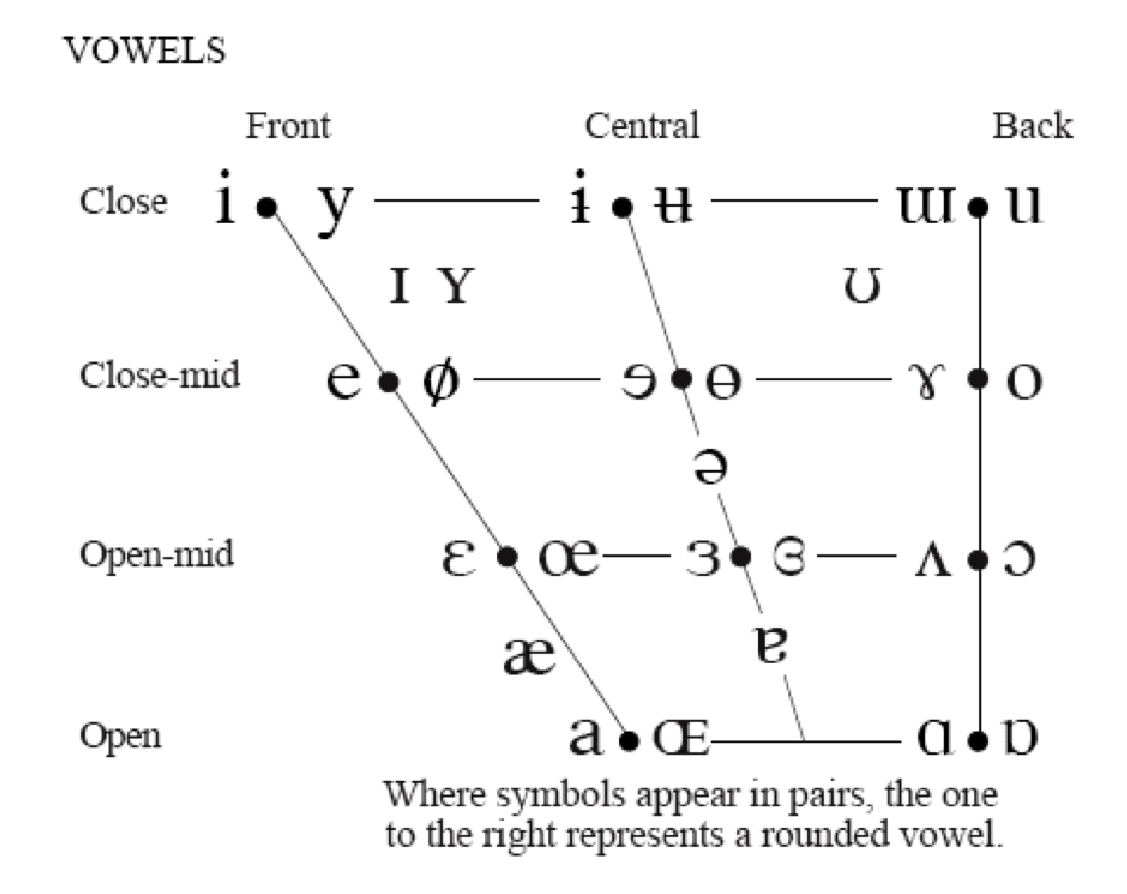
\includegraphics[width=6cm]{./includes/figures/ipa.eps}
\caption{The vowel chart used in the International Phonetic
Alphabet (IPA).}\label{fig:vowels}
\end{center}
\end{figure}

\subsection{Tables}

An example of a table is shown as
Table\textasciitilde{}\ref{tab:decibel}. Somewhat different styles are
allowed according to the type and purpose of the table. Colour should
not be used, but grey shading is allowed. There should be a margin of
6\textasciitilde points (pt) above and below the table.

The caption text may be above or below the table, but this should be
consistent throughout the submission. Left and right indentation of the
caption should be 0.5\textasciitilde cm.

\begin{table}[!ht]
  \begin{center}
  \begin{tabular}{|c|c|}
  \hline
  \rowcolor[gray]{.75}
  ratio    & Decibels\\
  \hline
  $1/1$    & $0$\\
  $2/1$    & $6$\\
  $3.16$   & $10$\\
  $1/10$   & $-20$\\
  $10/1$   & $20$\\
  $100/1$  & $40$\\
  $1000/1$ & $60$\\
  \hline
  \end{tabular}
  \caption{This is an example of a table showing Decibel (dB)
  ratios.}\label{tab:decibel}
  \end{center}
\end{table}

\subsection{Equations}

Equations should be placed on separate lines and numbered. An example of
an equation is \begin{equation}\label{eq:tzero}
T_0 = \frac{1}{f_0}.
\end{equation} Numbers of equations can be on the right or on the left
margin of the text column.

\subsection{Examples}

Examples from other languages can either be presented in the body text,
or, if referred to elsewhere or particularly long and complex, can be
put on a separate, numbered line, as should be done for equations.

\subsection{Phonetic fonts}

We recommend that you use the \textsc{tipa} package for IPA phonetic
symbols. For information about how to access Unicode fonts in the Word
template, see \cite{IPA-SIL} or \cite{IPA-KEYBOARD}. The font you use
must be embedded. Please remember to check this, e.g.~by inspecting the
``Document Properties --- Fonts'\,' in Acrobat Reader.

\subsection{Page numbering}

Page numbers will be added electronically to the document later.
\textit{Please do not add page numbers and please do not insert
any footers or headers!}

\subsection{References}

Please use just the reference number in square brackets. Formulations
with author names like ``\ldots~as Ladefoged \cite{Ladefoged:2003}
showed that \ldots'' are acceptable but not ``as shown in {[}Ladefoged,
3{]}'' or ``as shown in (Ladefoged {[}3{]})''.

References are to be numbered in alphabetical order. Please double-check
the final version of your paper with regard to the correct
correspondence of references to their numbers.

\subsection{Hyperlinks}

Links to URLs or email addresses should be formatted as normal text,
\textit{not} as hyperlinks and not blue or underlined etc. Usually
hyperlinks to web pages are listed in the references section. If
required, line breaks can be placed within URLs after slashes or dashes
(cf.\textasciitilde{}\cite{IPA-SIL,IPA-KEYBOARD}), but doublecheck that
no hyphens are inserted.

\subsection{Footnotes and endnotes}

If footnotes cannot be avoided they should appear as
endnotes.\footnote{This footnote appears here as an endnote.}

\section{Multimedia files}

Multimedia data that are part of the paper are to be embedded in the
submitted PDF; they cannot be submitted as supplementary data. Any
images are to be included in the paper as Figures (see Section 2.3
above). It is the authors' responsibility to check image quality ahead
of submission. Audio examples are to be embedded within the PDF. To do
this, authors can generate the PDF, and then embed the audio files using
Adobe Acrobat Professional, or other software that offers the same
outcome, so that the audio is included in the PDF. The presence of audio
data should be identified in the text.

We encourage authors to illustrate video data using still photographs
from the video, and to include them as figures in the PDF. We cannot
accept embedded video files, but authors are welcome to refer readers to
a URL on the internet where these can be viewed.

\section{PDF details}

PDF files submitted must comply with the following requirements:

\begin{enumerate}
\item all special fonts and symbols must be embedded in the PDF
  file so that correct rendering of the PDF does not depend on the
  fonts installed on the viewer's computer
\item there must be no
  password protection on the PDF file, i.e. PDF files must not be
  protected by PDF security in any way, i.e. content extraction,
  document assembly, high resolution printing etc. must not be
  forbidden
\item PDF files should not contain any colours, hyperlinks,
  multimedia or 3D content, and no JavaScript or forms
\item PDF files
  should be no larger than 5 MB.
\end{enumerate}

\section{Anonymity}

In ICPhS 2023 submissions, an anonymous reviewing process will be used.
This means that for the first submission the name(s) of the author(s)
and their affiliation(s) \emph{must not} be mentioned. In addition,
please refrain from using acknowledgements. Please also try to make your
own previous research as anonymous as possible. As an example: do not
write ``In our previous study \cite{Stevens:1999} we could show\ldots''
but ``As shown in \cite{Stevens:1999}\ldots''. Or refer to your own
published or otherwise widely known work, and to that of the other
authors, in the ``Julius Caesar style'', i.e.~in the third person (for
example: his work, her work, their work). Reference as ``anonymous''
only work that you or the other authors have submitted for publication,
but which has not yet been published, e.g.~\cite{Anonymous:submitted}.

Please make sure that no author details appear in the Document
Properties of the PDF file.
\emph{For the revised paper submission author details are of course needed}.
Acknowledgements and references to one's own work are possible as usual.

\section{Format of references}

References are formatted using the IEEE standard (available in various
reference management systems like Zotero or Mendeley). If you do not use
a reference management system, please use the examples provided for
monographs \cite{Fant:1960}, contributions to volumes
\cite{Stevens:1999}, journal articles \cite{Beattie/etal:1982}, articles
in conference proceedings \cite{Ladefoged:2003}. Abbreviations of
well-known conferences and journals are possible
\cite{Peterson/Barney:1952}. Software tools \cite{Boril/Skarnitzl:2016}
are referenced according to authors' instructions.

\section{R scripts}

You can use knitr code chunks like in any .Rmd document:

\begin{Shaded}
\begin{Highlighting}[]
\DecValTok{2} \SpecialCharTok{+} \DecValTok{2}
\end{Highlighting}
\end{Shaded}

\begin{verbatim}
## [1] 4
\end{verbatim}

This includes inline code: 2 + 2 = 4.

R scripts can be loaded as well:

\begin{Shaded}
\begin{Highlighting}[]
\FunctionTok{source}\NormalTok{(}\StringTok{"./includes/scripts/analysis.R"}\NormalTok{)}
\end{Highlighting}
\end{Shaded}

Which means you have access to any objects assigned in the script, like
Figure \ref{fig:ex_plot}:

\begin{Shaded}
\begin{Highlighting}[]
\NormalTok{cars\_plot}
\end{Highlighting}
\end{Shaded}

\begin{figure}[!h]
\caption{This is a figure caption.}\label{fig:ex_plot}


\begin{center}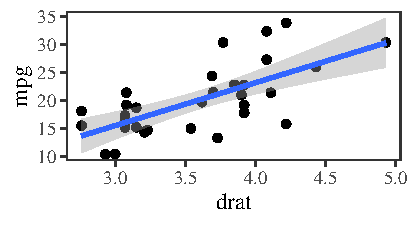
\includegraphics{main_files/figure-latex/ex_plot-1} \end{center}

\end{figure}

\bibliographystyle{./includes/bib/IEEEtran.bst}
\bibliography{./includes/bib/icphs2023.bib}

\theendnotes

\end{document}
